\documentclass[conference]{IEEEtran}
\IEEEoverridecommandlockouts
% The preceding line is only needed to identify funding in the first footnote. If that is unneeded, please comment it out.
% \usepackage[colorlinks=true, linkcolor=blue, urlcolor=blue, citecolor=blue, anchorcolor=blue]{hyperref}
\usepackage{hyperref}
% \usepackage{cite}
\usepackage{amsmath,amssymb,amsfonts}
\usepackage{algorithmic}
% \usepackage{graphicx}
\usepackage{graphicx,grffile}
% \let\oldincludegraphics\includegraphics
% \renewcommand{\includegraphics}[1]{\oldincludegraphics[width=0.5\textwidth,keepaspectratio]{#1}}
\ifCLASSOPTIONcompsoc
    \usepackage[caption=false, font=normalsize, labelfont=sf, textfont=sf]{subfig}
\else
\usepackage[caption=false, font=footnotesize]{subfig}
\fi
\usepackage{longtable,booktabs}
\usepackage{makecell, multirow}
\usepackage{textcomp}
% \usepackage[mathletters]{ucs}
\usepackage[utf8]{inputenc}
\usepackage[T1]{fontenc}
\DeclareUnicodeCharacter{0301}{\'e}
% \DeclareUnicodeCharacter{c2b4}{\'e}
% \UseRawInputEncoding

% \usepackage{lipsum}

\usepackage{listings}
\usepackage[dvipsnames]{xcolor}

\definecolor{codegreen}{rgb}{0,0.6,0}
\definecolor{codegray}{rgb}{0.5,0.5,0.5}
\definecolor{codepurple}{rgb}{0.58,0,0.82}
\definecolor{backcolour}{rgb}{0.95,0.95,0.92}

\lstdefinestyle{mystyle}{
    backgroundcolor=\color{backcolour},   
    commentstyle=\color{codegreen},
    keywordstyle=\color{magenta},
    numberstyle=\tiny\color{codegray},
    stringstyle=\color{codepurple},
    % stringstyle=\color{Peach},
    basicstyle=\ttfamily\footnotesize,
    breakatwhitespace=false,         
    breaklines=true,                 
    captionpos=b,                    
    keepspaces=true,                 
    numbers=left,
    numbersep=5pt,                  
    showspaces=false,                
    showstringspaces=false,
    showtabs=false,                  
    tabsize=2
}

\lstset{style=mystyle}

% \usepackage{minted}

\usepackage{tikz}

\usepackage[normalem]{ulem}
% Avoid problems with \sout in headers with hyperref
\pdfstringdefDisableCommands{\renewcommand{\sout}{}}
\usepackage[style=ieee,backend=bibtex]{biblatex}
\bibliography{as2.bib}

\providecommand{\tightlist}{%
  \setlength{\itemsep}{0pt}\setlength{\parskip}{0pt}
}

\def\BibTeX{{\rm B\kern-.05em{\sc i\kern-.025em b}\kern-.08em
    T\kern-.1667em\lower.7ex\hbox{E}\kern-.125emX}}

% 
\usepackage[noabbrev]{cleveref}
\newcommand{\mythead}[1]{\textbf{\thead{#1}}}

\begin{document}

\title{Popular Topic Mining from Blog Text\\
% {\footnotesize \textsuperscript{*}Note: Sub-titles are not captured in Xplore and should not be used}
% \thanks{Identify applicable funding agency here. If none, delete this.}
}

\author{\IEEEauthorblockN{Stone Fang (Student ID: 19049042)}
\IEEEauthorblockA{\textit{Computers and Information Sciences} \\
\textit{Auckland University of Technology}\\
Auckland, New Zealand \\
fnk7060@autuni.ac.nz}}

\maketitle

\begin{abstract}

Topic mining is an important way that provides insights of text data
about opinions and preference of people. In this project, a complete
topic mining solution is conducted, extracting two most popular topics
among 19,320 blog posts grouped by the demographic of authors. Topics
are generated from ranking objects that are mentioned in the dataset,
and two ranking methods are used, one using word-count and the other
based on TF-IDF. The result shows most topics are meaningful and
coherent, but the topic from two methods are very different. The quality
of mined topics are analysed and further discussions are presented.
Meanwhile, some topics have relatively lower quality and the causes are
analysed. In addition, with open issues and challenges pointed out,
future works and possible improvements are provided.

\end{abstract}

\begin{IEEEkeywords}
Topic mining, TF-IDF, Named entity recognition, Topic coherence
\end{IEEEkeywords}

\hypertarget{overview}{%
\section{Overview}\label{overview}}

People's concerns and opinions are important reference for innovations
of new products or services. However, accomplishing such task by humans
is expensive, time-consuming and difficult to scale. As a response, a
number of individuals and organisations are leveraging text mining
technologies to mining meaningful information from large volume of text
such as news media \autocite{jacobi_quantitative_2016}. Among a variety
of studies and applications, topic modelling is an important method to
extract hot topics which reflects public attention and opinion from
massive texts
\autocite{jacobi_quantitative_2016,waila_blog_2013,guo_mining_2012}.
However, effective method of extracting useful information from text on
the Internet remains an open challenge \autocite{guo_mining_2012}.

Evaluation of topics mined from text is another challenge, mostly due to
the lack of ground truth because topic modelling is an unsupervised
learning task \autocite{boyd-graber_care_nodate}.

The goal of this project is to mine most popular topics that people were
discussing from blog posts by utilising various text mining algorithms
and tools. Specifically, we will find two most popular topics for each
group in the following demographics:

\begin{itemize}
\tightlist
\item
  Males
\item
  Females
\item
  People 20 years old or younger
\item
  People older than 20
\item
  Everyone
\end{itemize}

The remainder of this article is organised as follows. In
\cref{sec:lit_review} related works on topic mining and evaluation will
be reviewed. The methodology of topic mining are detailed in
\cref{research-design}, while the results, analysis and evaluations are
presented in \cref{sec:result}. The works of this article are summarised
in \cref{conclusion} and open issues and future works are discussed in
\cref{open-issues-and-future-works}.

\hypertarget{sec:lit-review}{%
\section{Literature Review}\label{sec:lit-review}}

\textcite{jacobi_quantitative_2016} conducted an in-depth study of how
to apply topic modelling technologies on analysis of qualitative data in
academic research. This work also included a case study of analysis on
nuclear technology presented in New York Times from 1942.
\textcite{waila_blog_2013} conducted an analysis on blog text with
combination of topic modelling, NER, and sentiment analysis. Key themes
are extracted from the dataset, and topic perplexity is calculated for
evaluation. In addition, important entities such as person, place, and
organisation are also recognised and displayed by word cloud.
\textcite{guo_mining_2012} proposed a Frequent Pattern stream
(FP-stream) mining algorithm for hot topic discovery on Twitter. The
author argues that traditional clustering-based topic detection
algorithms are not suitable for the short, sparse, and fast-spreading
Twitter data. Experiments were carried out and the result showed the hot
topics and the trend of change over time.

\textcite{boyd-graber_care_nodate} provides a summary of topic
evaluation methods, which are divided into three categories: human
evaluation, diagnostic metrics, and coherent metrics. The first one
needs human effort so it is expensive and time-consuming, while the
other two can be calculated by computer without human interference.

\textbf{Human Evaluation} requires human involvement in the evaluation
task. One method in this category is accomplished by word intrusion
task. Specifically, a person will be presented by a list of words and is
asked to find an intruder in the meaning of not belonging to others. The
words list are constructed by first selecting highly possible words from
a topic, and then randomly choose one word with low probability in the
same topic but high probability in a different topic. If the intruders
are easily to be identified, then the topic is more likely coherent
\autocite{boyd-graber_care_nodate}.

\textbf{Diagnostic Metrics} only compute statistics of topics without
requirements of external knowledge source. Some methods in this category
are \autocite{boyd-graber_care_nodate}:

\begin{itemize}
\tightlist
\item
  Topic Size: measured by the sum of numbers of tokens belonging to a
  certain topic. Generally speaking, small topic size means low quality.
\item
  Word Length: average length of N most dominant words in a topic. The
  usefulness of this metric is corpus dependent.
\item
  Corpus Distribution Distance: A probability distribution can be
  derived from a topic over the vocabulary, and further normalised by
  global word count in the whole dataset. The distance between different
  topics reflects how much these topics are separated.
\end{itemize}

\textbf{Coherence Metrics} is a type of methods which automatically
compute score of topic coherence, and their accuracy is close to human
performance. The basic idea is measuring how a pair of words from top N
dominant words are associated \autocite{boyd-graber_care_nodate}. It is
formalised as

\[\mathrm{TC{\text-}f}(\mathbf{w}) = \sum_{i<j}{f(w_i, w_j)}, i, j \in \{1 ... N\}\]

where \(\mathbf{w} = \{w_1, w_2, ..., w_N\}\) is the list of N most
dominant words, and \(f\) is the scoring function of association between
two words. A typical value of N is 10. There are a variety of ways to
compute \(f\), such as counting the co-occurrence of two words, or
counting the number of documents containing both words. Two popular
implementations of \(f\) are Pointwise Mutual Information (PMI) and Log
Conditional Probability (LCP) \autocite{boyd-graber_care_nodate}.

\begin{align*}
\mathrm{PMI}(w_i, w_j) &= \log \frac{P(w_i, w_j)}{P(w_i) P(w_j)} \\
\mathrm{LCP}(w_i, w_j) &= \log \frac{P(w_i, w_j)}{P(w_j)}
\end{align*}

\textcite{fang_using_2016} proposed a metric based on Word Embeddings
(WE). Similar to Latent Semantic Analysis (LSA) which represents each
word as a real number vector obtained by Singular Value Decomposition
(SVD), the WE metric represents each word by a WE vector, and the
association scoring function is defined by cosine similarity of two
vectors:

\[f(w_i, w_j) = \mathit{cosine}(V(w_i), V(w_j))\]

\hypertarget{research-design}{%
\section{Research Design}\label{research-design}}

In this section the solution will be described in detail. First an
overview of the dataset is given, and then the algorithm of topic mining
is detailed.

\hypertarget{data-description}{%
\subsection{Data Description}\label{data-description}}

The dataset contains 19,320 files in XML format, each containing
articles of one person posted generally between 2001 and 2004. Metadata
of the bloggers includes gender, age, category, and zodiac. In addition,
the number of posts for each person are also counted. The result is
summarised by Fig. \ref{fig:data-desc}, which is created by Python
packages \texttt{pandas} and \texttt{matplotlib}. From this figure we
can acquire some basic statistics of the dataset, including

\begin{enumerate}
\tightlist
\item
  Gender: data samples are quite evenly distributed over both genders.
\item
  Age: most bloggers are younger than 30, almost of them under 20. On
  the other hand, there are two gaps around 20 and 30 which may implies
  some missing data points in the dataset
\item
  Gender and age group: since we divide the dataset by the author's age,
  it is beneficial to inspect some data distribution over age groups.
  Therefor, we plot the histogram for gender distribution for each age
  group and the data amounts for both genders in either age group are
  shown to be evenly distributed.
\item
  Zodiac: The distribution over zodiac is reasonable even.
\item
  Category: the most frequent category is unknown, which is trivial,
  while the second frequent one is student, far more than other
  categories.
\item
  Number of posts: most bloggers published less than 100 posts, while
  the peak appears at 10, which implies people are most likely to write
  around 10 posts.
\end{enumerate}

\begin{figure}[htbp]
  \centering
  \subfloat[Gender\label{gender}]{%
       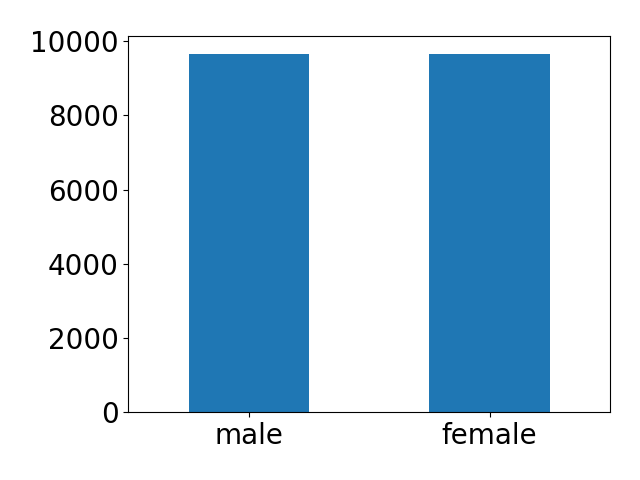
\includegraphics[width=0.48\linewidth]{img/show-gender.png}}
  %\hfill
  \subfloat[Age\label{age}]{%
        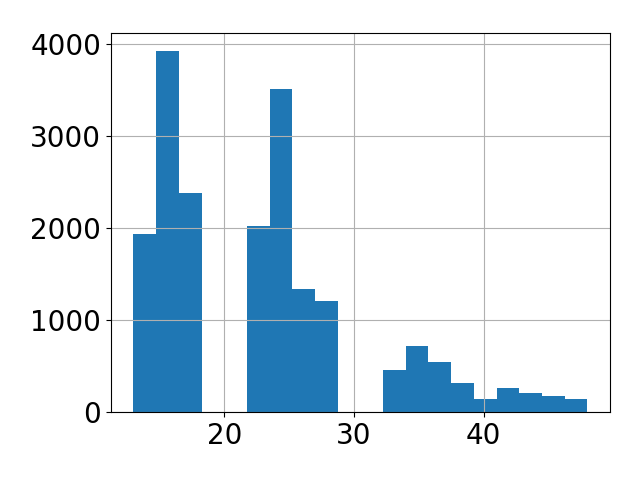
\includegraphics[width=0.48\linewidth]{img/show-age.png}}
  \\
  \subfloat[Gender-Age Group\label{category}]{%
       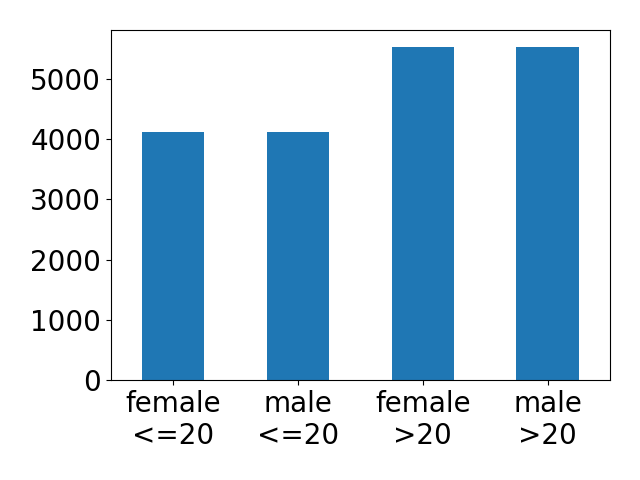
\includegraphics[width=0.48\linewidth]{img/show-gender-age.png}}
  %\hfill
  \subfloat[Zodiac\label{zodiac}]{%
       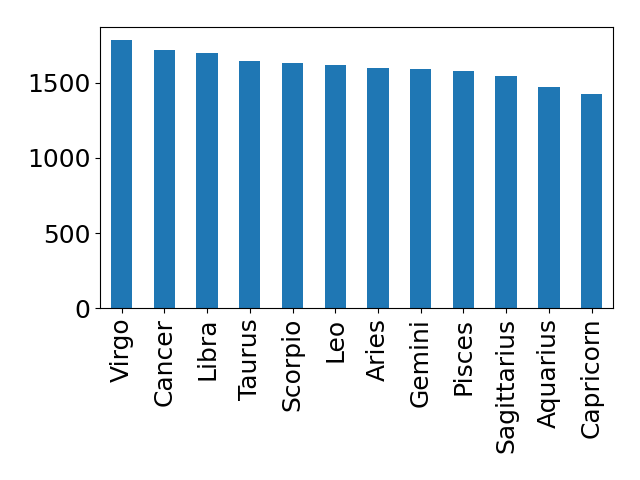
\includegraphics[width=0.48\linewidth]{img/show-zodiac.png}}
  \\
  \subfloat[Category\label{category}]{%
       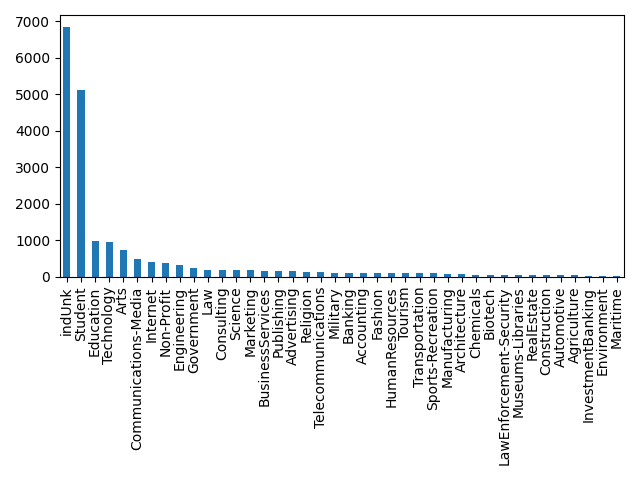
\includegraphics[width=0.48\linewidth]{img/show-category.png}}
  \subfloat[{Number of Posts}\label{num-posts}]{%
        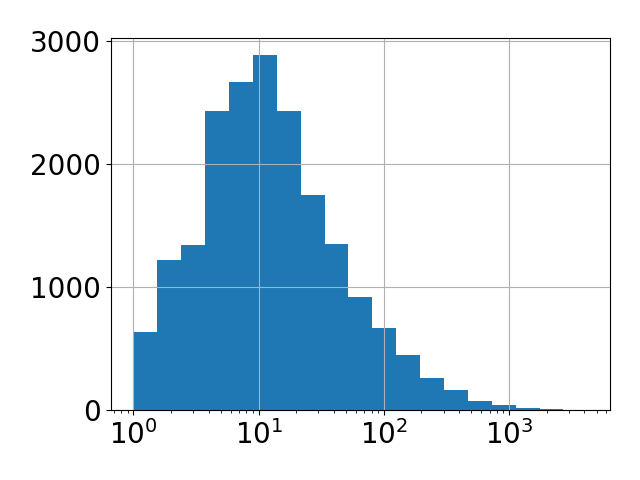
\includegraphics[width=0.48\linewidth]{img/show-blog-count.png}}
  \caption{Data Overview. Histogram over (a) gender (b) age (c) gender and age group 
      (d) zodiac (e) category (f) number of posts}
  \label{fig:data-desc}
\end{figure}

\hypertarget{topic-mining-algorithm}{%
\subsection{Topic Mining Algorithm}\label{topic-mining-algorithm}}

The general idea for mining popular topics used in this project is to
find the most significant ``things'' mentioned in the overall dataset,
as well as the closely related information.

The overall architecture of the algorithm is shown as Fig.
\ref{fig:overall}, and the details of each step are described in the
following subsections.

\begin{figure*}[htbp]
  \centering
  % \sffamily
  {
  %\fontfamily{phv}\selectfont
  \fontsize{9}{10}\selectfont
  % \fontsize{7}{7}\selectfont
  \def\svgwidth{0.98\textwidth}
  %  \resizebox{0.9\textwidth}{!}{\input{as2-algo.pdf_tex}}
    \input{as2-algo.pdf_tex}
  }
  \caption{Overall Architecture of Topic Mining Algorithm}
  \label{fig:overall}
\end{figure*}

\hypertarget{data-cleaning}{%
\subsubsection{Data Cleaning}\label{data-cleaning}}

Before applying any text mining techniques, it is important to do basic
data cleaning to improve data quality. In this step, a few operations
for preprocessing will be carried out based on the observations of the
dataset, with details as follows.

\begin{itemize}
\item
  \textbf{Problem}: At some place there is no whitespace between a
  punctuation and the word following it, which causes wrong
  tokenisation. Specifically, the punctuation might be tokenised with
  the following word as one token.

  \textbf{Solution}: Add whitespace after a punctuation if a word
  immediately follows it.

  \textbf{Example}:

  \begin{itemize}
  \tightlist
  \item
    \makebox[1cm][l]{input:}
    \texttt{\footnotesize I brought...stuff...like clothes}
  \item
    \makebox[1cm][l]{output:}
    \texttt{\footnotesize I brought... stuff... like clothes}
  \end{itemize}
\item
  \textbf{Problem}: Two or more consecutive quote symbols may cause
  wrong tokenisation.

  \textbf{Solution}: Replace two or more quotes as a double quote.
\item
  \textbf{Problem}: The unicode quote may affect tokenisation and
  stopwords matching.

  \textbf{Solution}: Replace unicode quote by ASCII quote.
\item
  \textbf{Problem}: The unicode quote may affect tokenisation and
  stopwords matching.

  \textbf{Solution}: Replace unicode quote by ASCII quote.
\item
  \textbf{Problem}: Characters that are usually not part of normal
  English text may disturb tokenisation and POS tagging.

  \textbf{Solution}: Remove invalid characters such as ``*'', ``\#'',
  and so on.
\item
  \textbf{Problem}: Sometimes people repeat a certain letter in a word
  for emphasis, but it will result in wrong words and also increase the
  vocabulary size.

  \textbf{Solution}: No English word has more than two consecutive
  appearances of the same letter, so three or more repetition of a
  letter is squeezed into two.

  \textbf{Example}:

  \begin{itemize}
  \tightlist
  \item
    \makebox[1cm][l]{input:}
    \texttt{\footnotesize going to be in deeeeep}
  \item
    \makebox[1cm][l]{output:} \texttt{\footnotesize going to be in deep}
  \end{itemize}
\end{itemize}

These operations are implemented by regex matching and substitution, or
simple text replacing. To use regex, the Python's \texttt{re} package
are imported.

\hypertarget{tokenisation}{%
\subsubsection{Tokenisation}\label{tokenisation}}

Tokenisation is usually the first step of all text mining pipelines,
which includes sentence and word tokenisation. Sentence tokenisation is
to split the whole text into sentences, while word tokenisation splits a
sentence into word or tokens. In this project we use \texttt{nltk}
package to do such task. This package provides two functions
\texttt{sent\_tokenize()} and \texttt{word\_tokenize()} for both
tokenisation. A document is first tokenised into sentences, and then
each sentence is tokenised into words. Finally, a document is
represented as list of lists, as each sentence is a list of words.

\hypertarget{pos-tagging}{%
\subsubsection{POS Tagging}\label{pos-tagging}}

Part-Of-Speech (POS) tagging is the second step following tokenisation.
In this step, each word is assigned by a POS tag. \texttt{nltk} provides
a handy function \texttt{pos\_tag()} to do this task. This function
works on sentence level, and maps each word into a tuple which is the
pair of word and POS tag.

\hypertarget{entity-extraction}{%
\subsubsection{Entity Extraction}\label{entity-extraction}}

In this project, a topic is defined as a ``thing'' or ``object''.
Therefore, in order to find the topics, we need to find all ``things''
or ``objects'' first. There are a few options to do this task, among
which two methods will be employed by this project: Named Entity
Recognition (NER) and parsing.

\hypertarget{ner}{%
\paragraph{NER}\label{ner}}

Named entities are ideal candidates of topics as they denote real-world
objects. \texttt{nltk} provides a function \texttt{ne\_chunk()} to
extract entities from sentences. The input of the function should be a
list of tokens with POS tags, which is another reason why POS tagging
should be done in previous step. The return value of this function is a
list of chunks, each of which is basically a list and may contain a
\texttt{label} attribute if it is a recognised entity. The entity type
can be acquired by \texttt{label()} and the entity itself should be
acquired by joining all the elements of the chunk.

\hypertarget{parsing}{%
\paragraph{Parsing}\label{parsing}}

Another way to extract objects is parsing by pre-defined patterns. For
example, it is reasonable to treat definite nouns as objects according
to the grammar, which can be extracted by matching of pattern ``the +
NOUN''. However, due to limited time, this technique is not used in the
experiment and might be considered in the future.

\hypertarget{stopwords-removal}{%
\subsubsection{Stopwords Removal}\label{stopwords-removal}}

Stopwords are most common words which carries no significant meanings.
Removing stopwords can reduce the size of data to be proceeded as well
as increase the result accuracy. \texttt{nltk} provides an
out-of-the-box stopwords collection, but the experiment shows that some
common words carrying no meaning are not included in the list. In order
to expand the stopword list, more words are collected from website
\footnote{\url{https://gist.github.com/sebleier/554280}}.

Stopwords removal is conducted after POS tagging and entity extraction
because these two steps are sequence model, which means their
performance rely on word order. If stopwords are removed before them, we
will get sentences which do not comply with English grammar. In
addition, stopwords removal are carried out on tagged documents as well
as entities extracted. Theoretically, stopwords cannot be entity, but
errors will happen in any POS tagging and NER model. Therefore, trying
to remove stopwords can reduce the error introduced in previous steps.

\hypertarget{stemming-and-lemmatisation}{%
\subsubsection{Stemming and
Lemmatisation}\label{stemming-and-lemmatisation}}

Stemming and lemmatisation are both techniques for text normalisation,
that is, convert an inflected word into its root form. However, stemming
and lemmatisation work in different way. Stemming removes suffix or
prefix from a word, returning a word stem which is not necessarily a
word. On the other hand, lemmatisation always looks for the lemma from
word variations with morphological analysis
\autocite{jabeen_stemming_2018}. For example, stemming against the
third-person singular form ``flies'' returns ``fli'', while
lemmatisation returns ``fly''. In this project, these two methods are
combined together to reach the maximum extent of word normalisation.

\texttt{nltk} provides various stemming algorithms such as
\texttt{PorterStemmer} and \texttt{LancasterStemmer}, and one
lemmatisation algorithm \texttt{WordNetLemmatizer}. In the code we use
\texttt{WordNetLemmatizer} followed by \texttt{PorterStemmer}.

\hypertarget{word-count-and-tf-idf}{%
\subsubsection{Word Count and TF-IDF}\label{word-count-and-tf-idf}}

After all ``objects'' have been extracted and normalised, the next step
is to find most popular ones as the most dominant topics. Popularity can
be defined in various ways, and in this project two approaches are used:
word count and Term Frequency-Inverse Document Frequency (TF-IDF). In
the first method, we simply count the appearances of each entity and get
the most two frequent ones. In the second method, we calculate the
TF-IDF value of each entity word, following the equation
\autocite{scott_tf-idf_2019}

\begin{align*}
\mathrm{TF{\text -}IDF}(t_i, d_j) &= 
\mathrm{TF}(t_i, d_j) \times \mathrm{IDF}(t_i) \\
& = \mathrm{TF}(t_i, d_j) \log \frac{N}{\mathrm{DF}(t_i)}
\end{align*}

\(\mathrm{TF}(t_i, d_j)\) is the Term Frequency of term \(t_i\) in
document \(d_j\), which is computed by count of \(t_i\) in \(d_j\)
divided by the total number of terms in \(d_j\). \(\mathrm{DF}(t_i)\) is
the Document Frequency, which is the number of documents that contains
\(t_i\). In order to avoid large IDF value for some terms only appearing
in a few documents, penalty is given to small DF values by adding a
smooth constant \({C}_{1}\) to DF

\[\mathrm{\overline{TF{\text -}IDF}}(t_i, d_j)
= \mathrm{TF}(t_i, d_j) \log \frac{N}{\mathrm{DF}(t_i) + {C}_{1}}\]

As we can see here, TF-IDF is a term-document-wise number so a term has
different TF-IDF values in different documents. In order to rank all
terms over the whole dataset, TF-IDF values of a term are averaged over
all documents as the score of that term. Similarly, penalty is also
given to terms having small DF values during the averaging process
because terms appears in too few documents are hardly to be defined as
popular. It is implemented by another smoothing constant \(C_2\) which
is not necessarily equal to \(C_1\). The effect of the penalty will be
further discussed in \cref{sec:tf-idf-analysis}.

\[\mathrm{score}(t_i)=\frac{1}{\mathrm{DF}(t_i) + {C}_{2}}
\sum_{d_j}\mathrm{\overline{TF{\text -}IDF}}(t_i, d_j)\]

Two different methods might return different results, which will be
compared and analysed in \cref{sec:result}.

\hypertarget{evaluation-method}{%
\subsection{Evaluation Method}\label{evaluation-method}}

Evaluation of topics is challenging due to its nature of unsupervised
learning. There are several topic evaluation approaches, including human
evaluation, diagnostic metrics, topic coherence, evaluation on
classification corpus. Human evaluation requires manual works so it is
costly and slow. Evaluation on classification corpus is a method using
labelled text classification corpus and checking the consistency between
topic words and class labels. Although we have categories in the
metadata for each document, a large portion of categories are labelled
as ``unknown'', so this approach is not suitable for this project.
Therefore, diagnostic and coherence metrics are chosen to evaluate the
result of the methodology. Details will be provided in \cref{sec:result}

\hypertarget{sec:result}{%
\section{Result, Evaluation and Analysis}\label{sec:result}}

This section will show the results generated from the methodology
described above, and provides evaluation and discussion of how good the
topics are. Two hottest topics are extracted for each demographic, and
each topic contains 10 words. In the TF-IDF-based method, penalty
parameters are set to \(C_1=C_2=100\). Due to the large volume of the
original dataset, the experiments were conducted with 5,000 and 10,000
documents randomly sampled out of the total 19,320 ones, and the results
demonstrated consistency. Therefore, in the following part of this
section, only results from 10,000 samples are presented. The complete
implementation is listed in \cref{appendix}, including two files, one
for topic mining algorithm and the other for result evaluation and
visualisation.

\hypertarget{result-and-evaluation}{%
\subsection{Result and Evaluation}\label{result-and-evaluation}}

The results are displayed as word cloud generated by \texttt{wordcloud}
and \texttt{matplotlib} package. Fig. \ref{fig:wc-tf} shows the topics
mined by word count while Fig. \ref{fig:wc-tfidf} shows that by TF-IDF.

\begin{figure}[pt]
  \centering
  \subfloat[Male\label{wc-tf-male}]{%
        \centering
       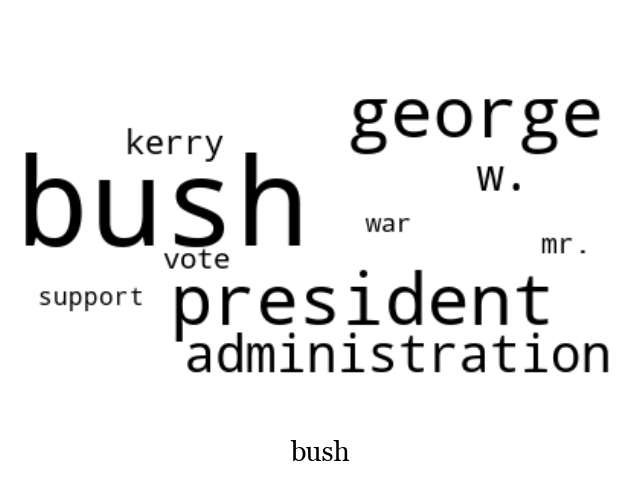
\includegraphics[width=0.42\linewidth]{img/male-tf-1.png}
       \hspace{0.35cm}
       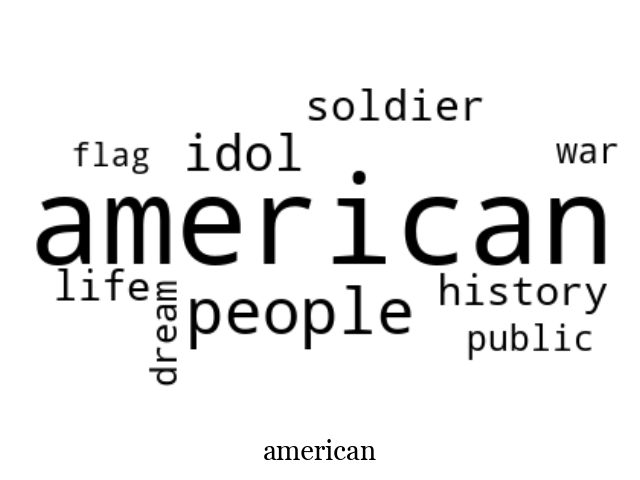
\includegraphics[width=0.42\linewidth]{img/male-tf-2.png}}
  \\[0.15cm]
  \subfloat[Female\label{wc-tf-female}]{%
        \centering
        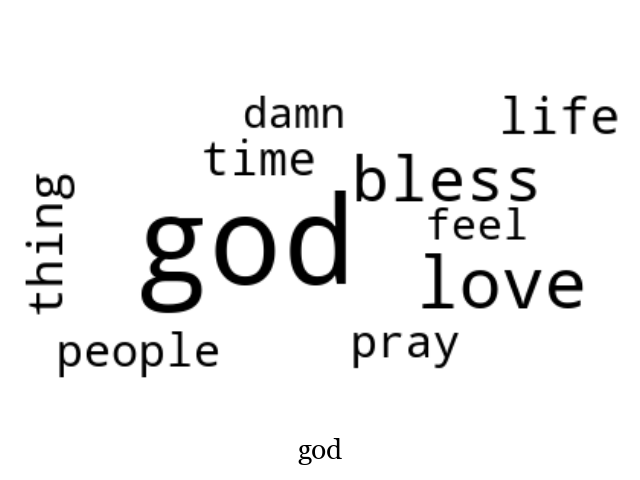
\includegraphics[width=0.42\linewidth]{img/female-tf-1.png}
        \hspace{0.35cm}
        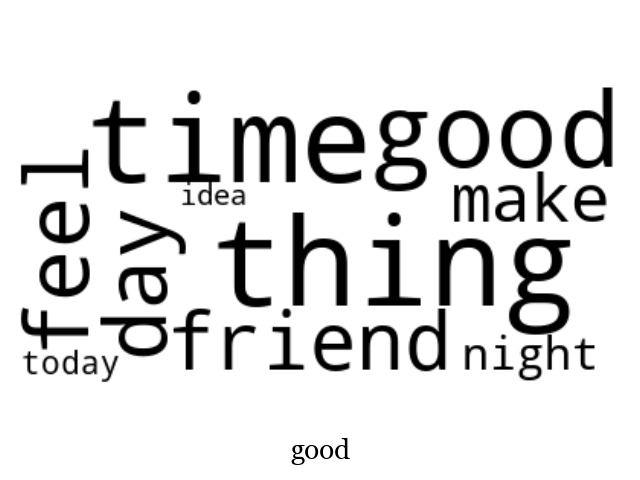
\includegraphics[width=0.42\linewidth]{img/female-tf-2.png}}
  \\[0.15cm]
  \subfloat[20 or younger\label{wc-tf-less}]{%
        \centering
        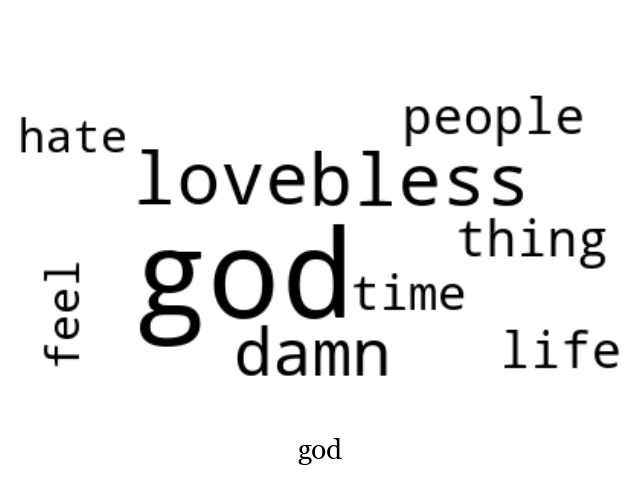
\includegraphics[width=0.42\linewidth]{img/less_or_20-tf-1.png}
        \hspace{0.35cm}
        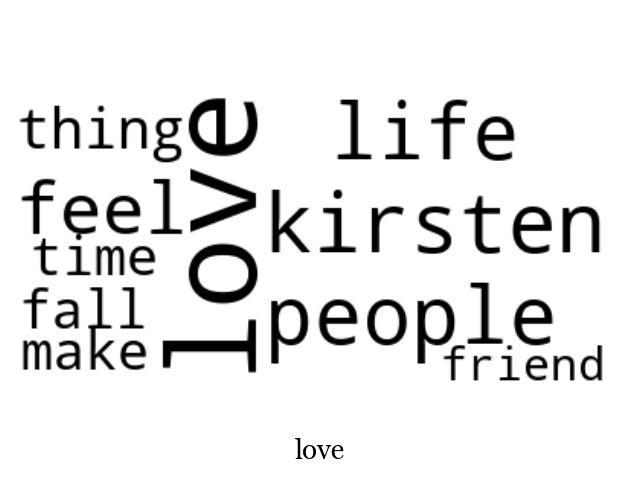
\includegraphics[width=0.42\linewidth]{img/less_or_20-tf-2.png}}
  \\[0.15cm]
  \subfloat[Over 20\label{wc-tf-over}]{%
        \centering
        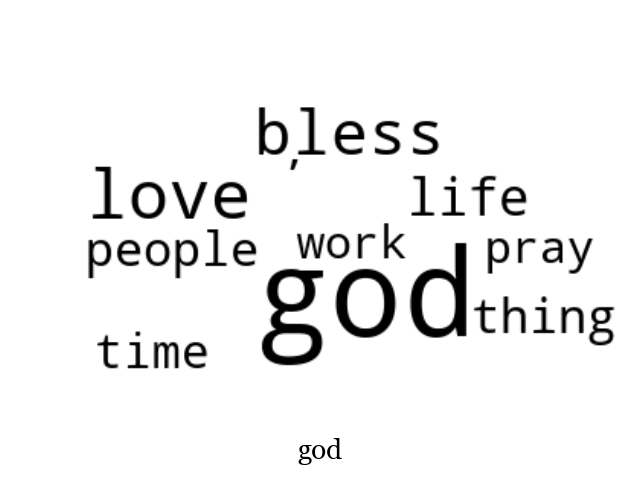
\includegraphics[width=0.42\linewidth]{img/over_20-tf-1.png}
        \hspace{0.35cm}
        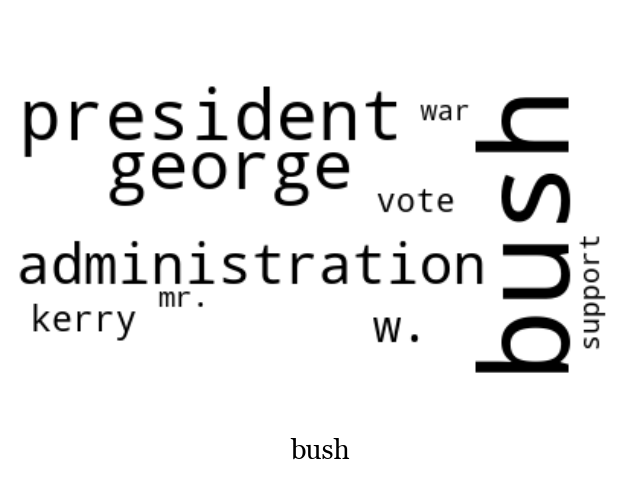
\includegraphics[width=0.42\linewidth]{img/over_20-tf-2.png}}
  \\[0.15cm]
  \subfloat[Everyone\label{wc-tf-all}]{%
        \centering
        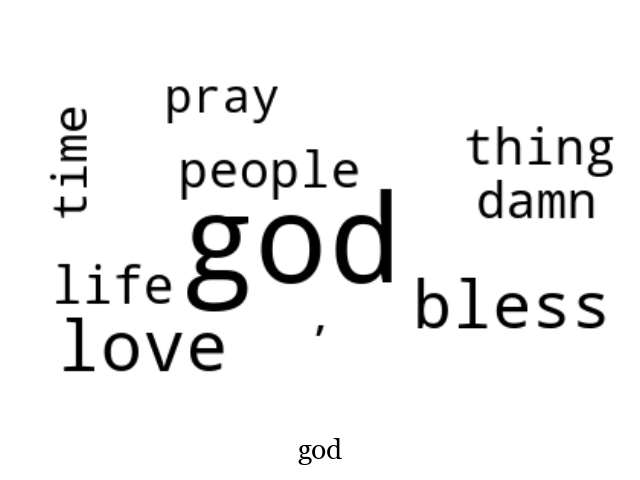
\includegraphics[width=0.42\linewidth]{img/all-tf-1.png}
        \hspace{0.35cm}
        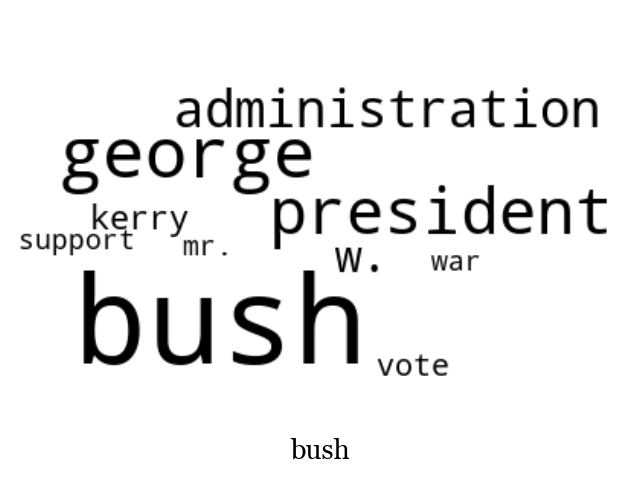
\includegraphics[width=0.42\linewidth]{img/all-tf-2.png}}
  \\[0.15cm]
  \caption{Topics mined by word count. (a) male (b) female (c) 20 or younger (d) over 20 (e) everyone}
  \label{fig:wc-tf}
\end{figure}

\begin{figure}[hpt]
  \centering
  \subfloat[Male\label{wc-tfidf-male}]{%
        \centering
       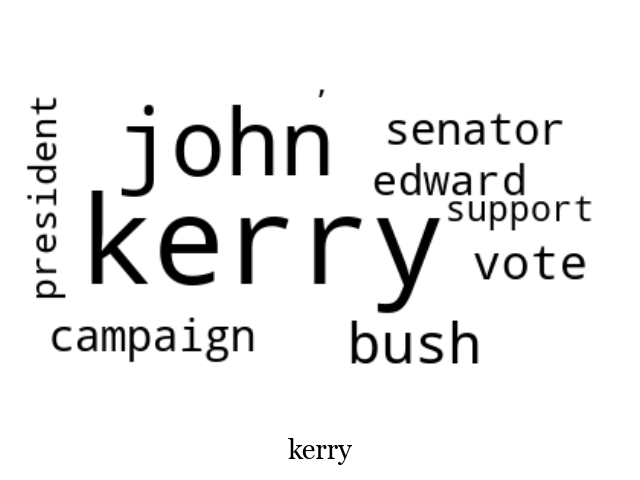
\includegraphics[width=0.42\linewidth]{img/male-tfidf-1.png}
       \hspace{0.35cm}
       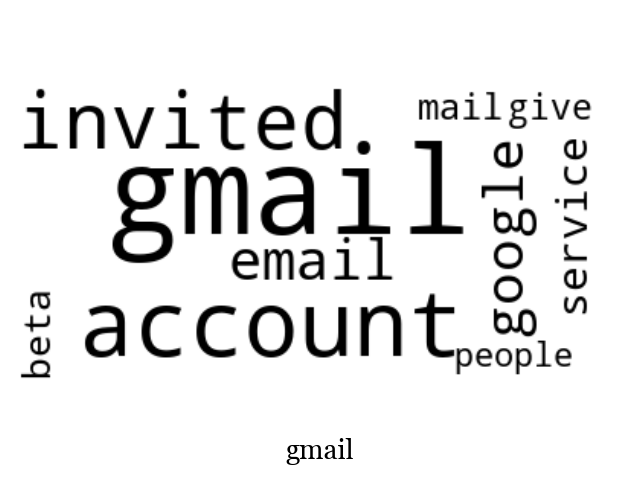
\includegraphics[width=0.42\linewidth]{img/male-tfidf-2.png}}
  \\[0.15cm]
  \subfloat[Female\label{wc-tfidf-female}]{%
        \centering
        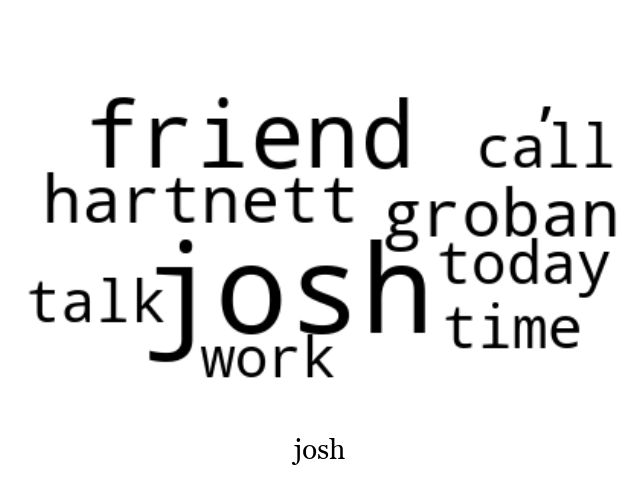
\includegraphics[width=0.42\linewidth]{img/female-tfidf-1.png}
        \hspace{0.35cm}
        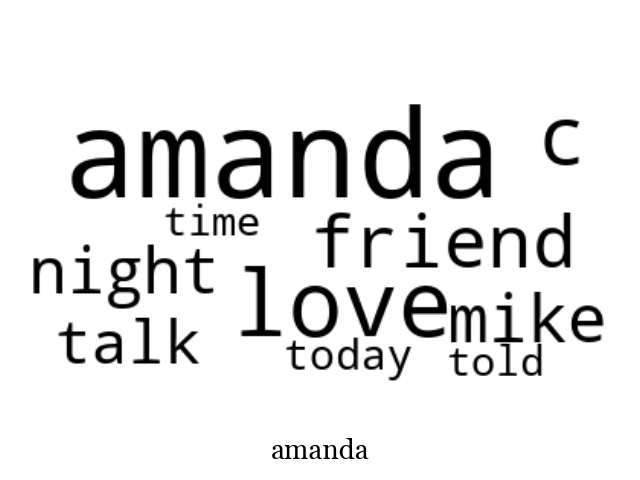
\includegraphics[width=0.42\linewidth]{img/female-tfidf-2.png}}
  \\[0.15cm]
  \subfloat[20 or younger\label{wc-tfidf-less}]{%
        \centering
        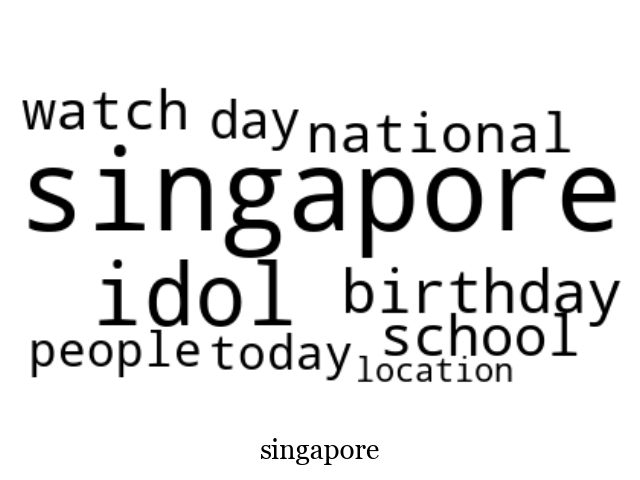
\includegraphics[width=0.42\linewidth]{img/less_or_20-tfidf-1.png}
        \hspace{0.35cm}
        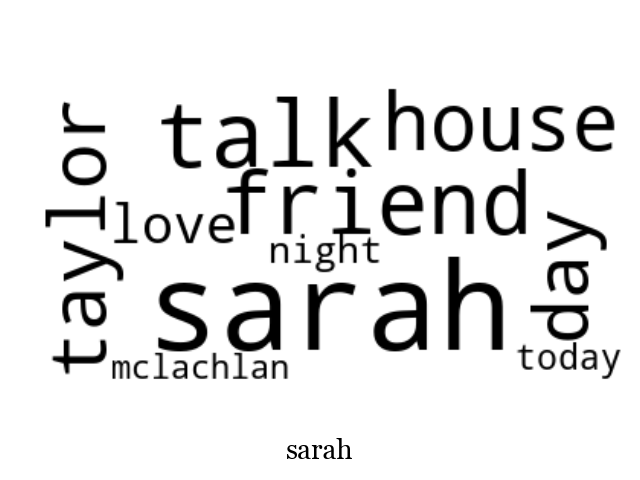
\includegraphics[width=0.42\linewidth]{img/less_or_20-tfidf-2.png}}
  \\[0.15cm]
  \subfloat[Over 20\label{wc-tfidf-over}]{%
        \centering
        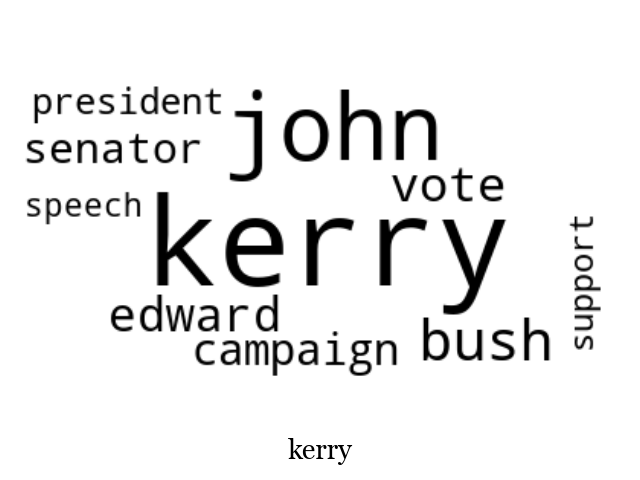
\includegraphics[width=0.42\linewidth]{img/over_20-tfidf-1.png}
        \hspace{0.35cm}
        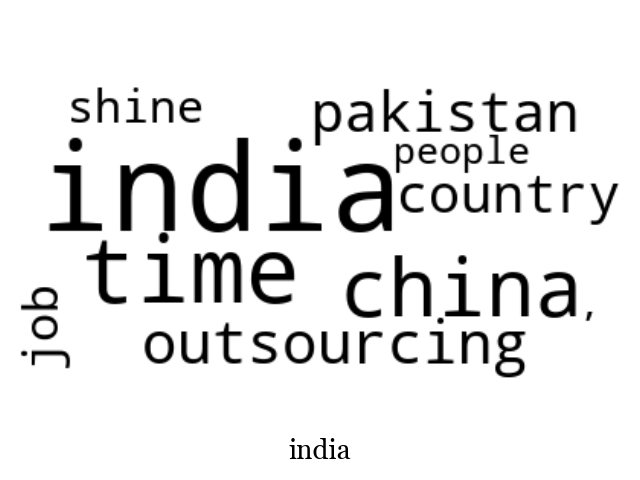
\includegraphics[width=0.42\linewidth]{img/over_20-tfidf-2.png}}
  \\[0.15cm]
  \subfloat[Everyone\label{wc-tfidf-all}]{%
        \centering
        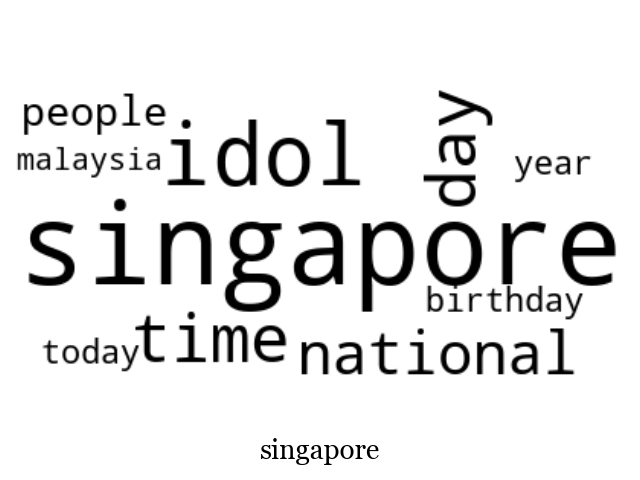
\includegraphics[width=0.42\linewidth]{img/all-tfidf-1.png}
        \hspace{0.35cm}
        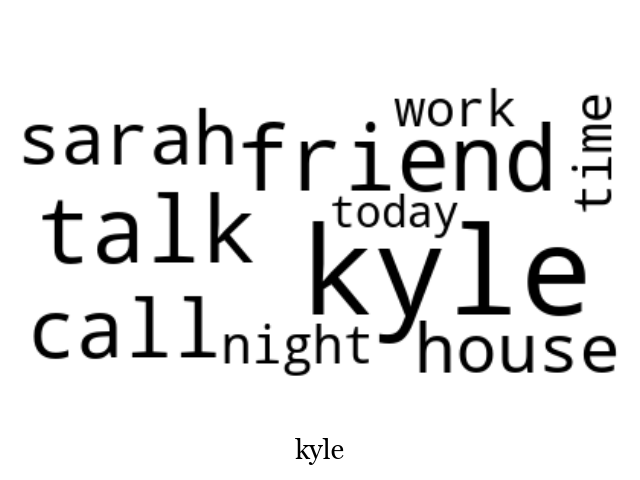
\includegraphics[width=0.42\linewidth]{img/all-tfidf-2.png}}
  \\[0.15cm]
  \caption{Topics mined by TF-IDF. (a) male (b) female (c) 20 or younger (d) over 20 (e) everyone}
  \label{fig:wc-tfidf}
\end{figure}

\begin{table}[pt]
\caption{Metrics for Word Count}
\label{tbl:eval-tf}
\begin{center}
\small
  \begin{tabular}{|c|c|r|l|l|l|} 
  \hline
  \multirow{2}{*}[-7pt]{\centering\textbf{\thead{Demographic}}} 
      & \multirow{2}{*}[-7pt]{\centering\textbf{\thead{Topic}}} 
      & \multicolumn{2}{c|}{\textbf{\thead{Diagnostic}}} 
      & \multicolumn{2}{c|}{\textbf{\thead{Coherence}}}  \\
  \cline{3-6}
  & & \textbf{\thead{Topic\\Size}} & \textbf{\thead{Word\\Length}} & \textbf{\thead{LSA}} & \textbf{\thead{GloVe}}  \\
  \hline
  \input{metrics-tf.tex}
\end{tabular}
\end{center}
\end{table}

\begin{table}[hpt]
\caption{Metrics for TF-IDF}
\label{tbl:eval-tfidf}
\begin{center}
\small
  \begin{tabular}{|c|c|r|l|l|l|} 
  \hline
  \multirow{2}{*}[-7pt]{\centering\textbf{\thead{Demographic}}} 
      & \multirow{2}{*}[-7pt]{\centering\textbf{\thead{Topic}}} 
      & \multicolumn{2}{c|}{\textbf{\thead{Diagnostic}}} 
      & \multicolumn{2}{c|}{\textbf{\thead{Coherence}}} \\
  \cline{3-6}
  & & \textbf{\thead{Topic\\Size}} & \textbf{\thead{Word\\Length}} & \textbf{\thead{LSA}} & \textbf{\thead{GloVe}} \\
  \hline
  \input{metrics-tfidf.tex}
\end{tabular}
\end{center}
\end{table}

For evaluation of the quality of topics, we computed two diagnostic
metrics, topic size and word length, and two coherence metrics, LSA and
Word Embedding. The LSA vectors are provided by
\autocite{rus_semilar_nodate}. The pre-trained GloVe
\autocite{pennington2014gloVe} word vectors with 100 dimension size are
used as word embeddings. The metrics are summarised in
\cref{tbl:eval-tf} and \cref{tbl:eval-tfidf} for two methods,
respectively.

\hypertarget{analysis}{%
\subsection{Analysis}\label{analysis}}

In this section we will first conduct in-depth analysis on topics from
both methods, and then compare these two results and discuss the pros
and cons for each method.

\hypertarget{method-of-word-count}{%
\subsubsection{Method of Word Count}\label{method-of-word-count}}

Most topics are meaningful and coherent. For instance, the topic
``bush'' is about U.S. president George W. Bush and relative concepts,
such as his rival John Kerry in 2004 U.S. president election and the
Iraq War began in 2003. The word length is relatively heigh and both LSA
and GloVe coherences are also high. However, the topic size is low and
the reason could be that it is specific on politics. Another example is
``god'' which appears in multiple demographics. Though the word length
is low, the topic size and coherence are high. We can also see that the
keywords in this topic are meaningful and relavent, such as ``love'',
``life'', ``people'', ``bless'', and so forth. On the other hand, the
topics ``love'' and ``good'' are too generic, thus have lower coherence
scores.

\hypertarget{sec:tf-idf-analysis}{%
\subsubsection{Method of TF-IDF}\label{sec:tf-idf-analysis}}

The topics ranked by TF-IDF are different from word count. A topic
relavent to the result from word count is ``kerry'', which we can tell
from the keywords respresents U.S. Senator John Kerry and also the
Democratic nominee for presidency competing with George W. Bush. The
coherence of this topic is also high. Several other topics are about
artists, singers or movie stars, but the qualities vary. For example,
the topic ``sarah'' contains Sarah McLachlan. By contrast, the topic
``josh'' actually contains two people, Josh Groban and Josh Hartnett, so
it should be two topics. Accordingly, the coherence for topic ``josh''
is very low. However, some topics are hard to tell what they represent,
such as ``amanda'' and ``kyle'', which are pobably just common names in
English world.

Two other meaningful topics are ``singapore'' and ``india'', which are
likely to be created by users from these two contries. An evidence of
the significant number of Singaporean users is that the word ``haiz'' as
a common saying of ``sigh'' in Singaporean English came out as a high
ranked topic candidate before it was filtered out as a stopword. The
``india'' topic is more informative, which is telling us about the
important job outsourcing in India which is consistent to our knowledge.
However, the coherence metrics are not signifcantly high, which could be
distracted by not-so-relavent words such as ``today'', ``time'',
``day''. The ``india'' topic has less distracting words and higher LSA
coherence score, but the GloVe score is low, which is a possibile issue
of WE coherence metrics.

The topic ``gmail'' is a different case. From human's point of view, it
is a meaningful topic representing the launch of beta release of
Google's mail service at 1 April, 2004. However, both coherence scores
are quite low, which may implies some drawbacks in the metrics
definition.

\hypertarget{comparison}{%
\subsubsection{Comparison}\label{comparison}}

As can be seen from above results and analysis, the topics mined by two
methods are highly different and share little in common. The difference
comes from difference natures of these two methods.

The word-count-based method takes the ``thing'' mentioned the most times
as the most popular one. This approach is simple and straightforward,
and consistent to humans' concept of popularity. The more widely
spreaded across the dataset an object is, the more likely it is selected
as the hottest topic. That is why we got very general topics such as
``god'', ``good'', ``love'', as well as ``bush'' during the period of
U.S. president election.

On the other hand, the TF-IDF-based method gives larger score on less
frequent terms. However, if some term is mentioned too few times, it
cannot be a hot topic. Therefore, penalty is given to such terms to make
them lower ranked, leading to a trade-off between specialty and
frequency and the choice of parameter representing the penalty is more a
trick. Experimental shows that if the penalty is too high, the result
from TF-IDF is quite similar to that from word count; but if it is too
small, result is more likely to be some concept only mentioned in a few
document. Generally speaking, this approach prefers topics that are
frequently mentioned in a certain subgroup of people, for example, pop
and movie stars, and people from a specific country such as Singapore
and India.

Each method has its own advantages and disadvantages, but some topics
from word-count- based method may be less valuable because they are too
general. For instance, the topic ``good'' or ``love'' hardly provides
any value to marketing or product decision-making because it is somthing
that people are always talking about. By contrast, though the result
from TF-IDF-based method may be only popular in a small group of people,
it does provide insights into the opinion of that group. However, some
topic from the first method is also valuable, such as the topic ``bush''
capturing people and events related to then U.S. president George W.
Bush.

\hypertarget{conclusion}{%
\section{Conclusion}\label{conclusion}}

This project has designed and implemented a complete solution to mine
most popular topics from blogs. A variety of text mining technologies
are employed and combined together to reach the goal. In order to rank
topics from a candidate list formed by objects, two methods are used:
word-count-based and TF-IDF-based. The results are displayed by word
cloud and metrics are computed and summarised. The results are also
discussed, compared and evaluated in detail, and the retionale is given.
Further and in-depth analysis is also provided.

\hypertarget{open-issues-and-future-works}{%
\section{Open Issues and Future
Works}\label{open-issues-and-future-works}}

There are still a few open issues remaining in the solution which can be
improved by future work or changed if re-do this project.

An important concern is the quality of NER which has big influence on
the final results. The NER result is used for topic candidate generating
and wrong entities will cause wrong topics. The experiment showed that
the quality of NER is moderate and needs improvement. To do that we can
use other NER tools such as \texttt{spaCy} and combine the results for
better performance.

Data cleaning is also an important stage in the whole algorithm. The
data from internet is quite noisy. Though we employed several
pre-processing to clean it, there are still many noises. For example,
the advertisment in blog posts is a great inteferential factor because
the same advertisment appears in the text very frequently thus looks
like a popular topic.

Spell checking is another means that can be used as an improvement
because blog text as a kind of informal text often has many spelling
errors which makes it more difficulty to do POS tagging and NER
correctly. There a few spell checking packages in Python, but they
requires very long time to finish large dataset, so they are not
included in the current methodology. Therefore, faster and more scalable
spell checking algorithms is another direction of future work.

% \lipsum[1-50]

% \bibliography{ass1}{}
% \bibliographystyle{IEEEtran}

\printbibliography


\onecolumn

\appendix [Source Code in Python]
\label{appendix}

% \section{Source Code in Python}
% \label{source-code}

\subsection{Code for topic mining}

\lstinputlisting[language=Python]{as2.py.tmp}

% \newpage

\subsection{Code for analysis, evaluation and visualisation}

\lstinputlisting[language=Python]{as2-eval.py.tmp}

% \begin{minted}[mathescape,
%     linenos,
%     numbersep=5pt,
%     gobble=2,
%     frame=lines,
%     framesep=2mm]{csharp}
% string title = "This is a Unicode \pi in the sky"
% /*
% Defined as $\pi=\lim_{n\to\infty}\frac{P_n}{d}$ where $P$ is the perimeter
% of an $n$-sided regular polygon circumscribing a
% circle of diameter $d$.
% */
% const double pi = 3.1415926535
% \end{minted}


% \lipsum[1-50]


\end{document}
